\section{Signalverarbeitung}
\label{sec: Modbus RTU}

\subsection{RS232}
\label{subsec:RS232}

\subsection{RS485-Kommunikation über Modbus RTU}
\label{subsec:RS485}

Modbus RTU ist ein Kommunikationsprotokoll, das entweder über RS485, RS232 oder Ethernet kommuniziert. Modbus RTU ist, wie viele andere Feldbusse, nach der Norm IEC 61158 \footnote{\textit{Digital data communication for measurement and control - Fieldbus for use in industrial control systems}} weltweit standardisiert.

Die Vorteile von Feldbussen sind der geringe Verkabelungsaufwand und die Möglichkeit der Eigendiagnose durch das System selbst. Ein Feldbus-System bietet eine hohe Flexibilität gegenüber Erweiterungen oder Änderung des Netzwerkes. Eine Festlegung auf Messbereiche der Sensoren ist nicht notwendig. Ein weiterer Vorteil ist die Möglichkeit der Abfrage unterschiedlicher Messwerte, wie zum Beispiel Temperatur und Druck, von einem Sensor. Die hohe Zuverlässigkeit und hohe Kompatibilität von verschiedenen Sensortypen ist ein weiterer großer Vorteil.

Die Nachteile eines Feldbusses sind die komplexeren Netzwerkstrukturen und -abläufe. Für eine erfolgreiche Implementierung eines Feldbus-Systems wird ein höher qualifiziertes Personal benötigt. Des Weiteren erfordert eine Abfrage der Sensoren meist eine größere Reaktionszeit. Sensoren mit  entsprechender Feldbustechnik sind häufig teurer als Sensoren, die mit analoger Datenübertragung ausgestattet sind. Eine Beschädigung des Kabels kann in manchen Fällen zum Ausfall des kompletten Feldbusses und dessen Sensoren führen. Redundante Netzwerke sind folglich wünschenswert, jedoch nicht immer umsetzbar. 

\begin{figure}[htb]
 \centering		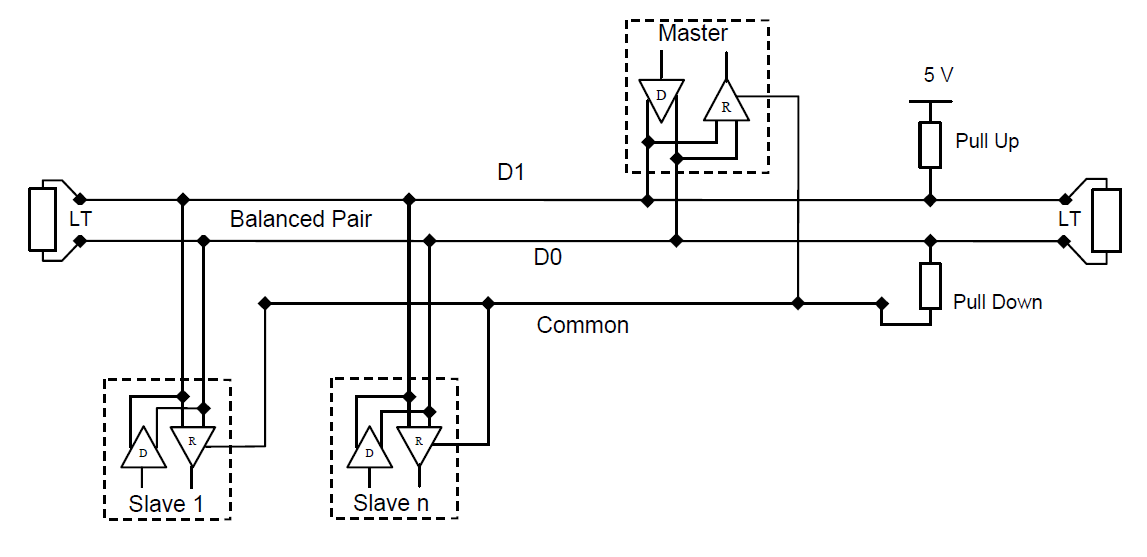
\includegraphics[width=0.94\textwidth]{Pictures/TopologieModbus.png}
 \caption{Zwei-Kabel-Topologie eines Modbus RTU-Feldbusses \citep{MODBUS.ORG2002}  }
 \label{fig:ZweiKabelModbus}
 \end{figure} 
 
Für den Modbus RTU wird nach \citep{MODBUS.ORG2002} eine Serienschaltung der Hardware-Komponenten (engl. \textit{Daisy Chain}) empfohlen. Die Komponenten sind in dieser Topologie in einer Kette verbunden. Ein Netzwerk besteht zu jeder Zeit aus einem Master und multiplen Slaves. Zunächst schickt der Master einen Befehl an einen Slave. Der Slave setzt den Befehl um und schickt dem Master seine Antwort. Die Befehle über die Sendekabel werden nur vom Master empfangen. Die Befehle über das Empfängerkabel werden hingegen nur von den Slaves empfangen.
 
Ein Modbus RTU kann über ein Vier- oder Zwei-Kabel-Topologie verfügen. Ein Vier-Kabel-Topologie verfügt über zwei paarweise Kabel, über die entweder gesendet oder empfangen wird. Die Kabel tragen nach der \textit{EIA/TIA-485 Standard} die Namen $D0$ und $D1$ und werden auch positive und negative \textit{Polarität} genannt. In beiden Topologiefällen können bis zu 32 Slaves angeschlossen werden und bis auf eine Entfernung von größer 1000 m betrieben werden. 

Zusätzlich zu den vier bzw. zwei Kabeln wird ein weiteres Kabel, das \textit{Common}, benötigt. Es stellt ein gleiches Spannungsniveau für alle Slaves sicher. Elektromagnetische Störungen beeinflussen die Datenleitungen ($D0$ und $D1$) und das $Common$-Kabel im gleichen Maße. Die Potentialdifferenz von D1 und D0 zu Common ist folglich konstant. Serielle Bits (0 oder 1) werden mittels Potentialdifferenzen zwischen $D0$ und $D1$ gesendet. Diese Verkabelungsart ist sehr unanfällig gegenüber elektromagnetischer Störsignale. 

Abbildung \ref{fig:ZweiKabelModbus} zeigt eine typische Zwei-Kabel-Topologie mit Abschlusswiderständen (engl. \textit{Line-Termination} (LT)), einem \textit{Pull-up}- und \textit{Pull-Down}-Widerstand.  Abschlusswiderstände (meist 150 $\Omega$, 0,5 W) werden an den zwei Enden der Linientopologie vorgesehen und dienen zur Reduzierung von Signalreflexionen am Ende der Leitungen. Diese können zu Fehlern in der Kommunikation führen. 
Es wird ein \textit{Pull-Up} und ein \textit{Pull-Down} mittels Widerstand zwischen 450 und 650 Ohm durchgeführt. Ein \textit{Pull-Up} zieht die $D1$-Datenleitung auf ein Ruhepotential von 5 V und ein \textit{Pull-Down} die $D0$-Datenleitung auf das Ruhepotential des \textit{Common}-Leiters (meist 0 V).

Das Bussystem RS485 erlaubt es bis zu 32 Sensoren auf einer Entfernung von theoretisch 1000 m anzuschließen.